\documentclass{beamer}

\usetheme[progressbar = frametitle]{metropolis}

\usepackage{tikz}
\usepackage{biblatex}
\usepackage[plain]{fancyref}

\usetikzlibrary{shapes,arrows,positioning,calc}

\addbibresource{../docs/breastMassDetection.bib}

\title{A Deep Learning Approach for Breast Cancer Mass Detection : A Review}

\author{
  Omar Emara (20180364), Omar Khaled (20180367),
  Ibrahim Magdy (20180014), Ahmed Nasser (20160052), Moataz Nasr (20180614)
}
\date{}

\begin{document}

\maketitle

\begin{frame}{Table Of Contents}
  \setbeamertemplate{section in toc}[sections numbered]
  \tableofcontents[hideallsubsections]
\end{frame}

\section{Introduction}

\begin{frame}{Context}
  \begin{itemize}
    \item Breast cancer is one of the fastest growing types of cancer.
    \item Early detection is of essence in death prevention.
    \item Detection is typically done by \alert{Mammography Screening}.
  \end{itemize}
\end{frame}

\begin{frame}{Abstract}
  \begin{itemize}
    \item Advances in machine learning and the greater availability of public
      mammography datasets allowed researches to develop machine learning
      models that achieve greater detection accuracy.
    \item We review one such research paper \alert{\autocite{Fathy2019}}.
    \item A TensorFlow implementation is presented.
  \end{itemize}
\end{frame}

\begin{frame}{Summary}
  \begin{itemize}
    \item The paper describe a \alert{Transfer Learning} approach to detect the
      existence of breast masses in mammogram images.
    \item Model is based on a pre-trained \alert{ResNet-50} model similar to
      the one described in \autocite{He2016}.
    \item Breast masses are localized using \alert{Class Activation Map (CAM)}
      based on the algorithm described in \autocite{Zhou2016}.
  \end{itemize}
\end{frame}

\section{Dataset}

\begin{frame}{Reference Dataset}
  \begin{itemize}
    \item The paper utilizes a subset of the \alert{Digital Database for
      Screening Mammography (DDSM)} published in \autocite{Bowyer1996}
      and \autocite{Heath1998}.
    \item The paper selected 2517 mammograms for training, 629 for validation,
      and 786 for testing.
  \end{itemize}
\end{frame}

\begin{frame}{Utilized Dataset}
  \begin{itemize}
    \item The size of the dataset was too large for us to download and utilize.
    \item Curated versions exists, such as the \alert{CBIS-DDSM} dataset
      presented in \autocite{Lee2017}. Still too large.
    \item We used a smaller version published in \autocite{Luka2020}.
  \end{itemize}
\end{frame}

\begin{frame}{Dataset Description}
  \begin{itemize}
    \item Mammograms are cropped around the \alert{Region Of Interest (ROI)}
      available in the meta-data of the original dataset.
    \item Mammograms have a resolution of $900 \times 900$.
  \end{itemize}
\end{frame}

\section{Preprocessing}

\begin{frame}{Segmentation}
  \begin{itemize}
    \item The breast region is masked and tightly cropped around the mask.
    \item The mask is generated using the \alert{ST Segmentation} technique
      described in \autocite{Pertuz2014}.
    \item Unnecessary for our dataset because it is already cropped around the
      ROI.
  \end{itemize}
\end{frame}

\begin{frame}{Model Suiting}
  \begin{itemize}
    \item The mammograms are processed to be suitable for the ResNet-50 model.
    \item The model requires the images to be of resolution \alert{$224 \times
      224$} with three color channels. Done using the Python \texttt{Pillow}
      module.
    \item The model require the images to have zero centered values relative
      to the ImageNet dataset. Done using the \texttt{preprocess\_input}
      function of the \texttt{resnet} module of Tensorflow.
  \end{itemize}
\end{frame}

\section{Model}

\begin{frame}{Architecture}
  \begin{itemize}
    \item A ResNet-50 model is created without the last prediction layer.
    \item A dense layer of a single unit with a sigmoid activation function is
      connected to the \alert{Global Average Pooling} layer to act as a
      prediction layer.
  \end{itemize}
\end{frame}

\begin{frame}{Architecture Diagram}
  \begin{figure}
  \begin{center}
  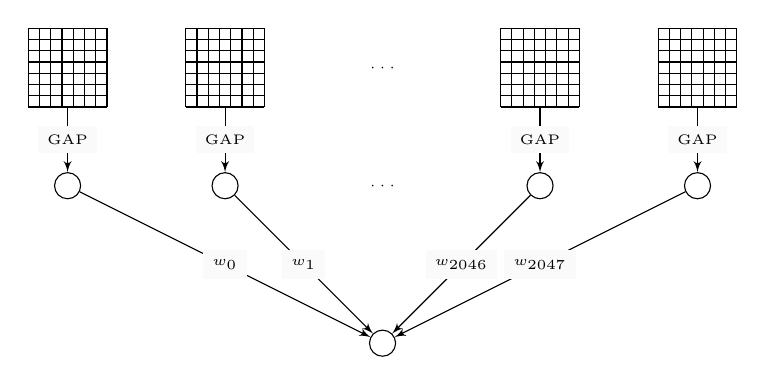
\begin{tikzpicture}[auto, node distance = 3cm, > = latex', font = \tiny]
    \tikzset{
      neuron/.style = {draw, circle},
      weight/.style = {fill = black!2, anchor = center},
    }
    \node [neuron] (output) at (0, -1) {};
    \node [neuron] (gap0) at (-4, 1) {};
    \node [neuron] (gap1) at (-2, 1) {};
    \node (gap2) at (0, 1) {$\cdots$};
    \node [neuron] (gap3) at (2, 1) {};
    \node [neuron] (gap4) at (4, 1) {};

    \draw [->] (gap0) -- node[weight]{$w_{0}$} (output);
    \draw [->] (gap1) -- node[weight]{$w_{1}$} (output);
    \draw [->] (gap3) -- node[weight]{$w_{2046}$} (output);
    \draw [->] (gap4) -- node[weight]{$w_{2047}$} (output);

    \draw[step = 0.142857143, shift = {(-4.5, 2)}] (0, 0) grid (1, 1);
    \draw[step = 0.142857143, shift = {(-2.5, 2)}] (0, 0) grid (1, 1);
    \node at (0, 2.5) {$\cdots$};
    \draw[step = 0.142857143, shift = {(1.5, 2)}] (0, 0) grid (1, 1);
    \draw[step = 0.142857143, shift = {(3.5, 2)}] (0, 0) grid (1, 1);

    \draw [->] (-4, 2) -- node[weight]{GAP} (gap0);
    \draw [->] (-2, 2) -- node[weight]{GAP} (gap1);
    \draw [->] (2, 2) -- node[weight]{GAP} (gap3);
    \draw [->] (4, 2) -- node[weight]{GAP} (gap4);
  \end{tikzpicture}
  \end{center}
  \caption{
    The last three layers of the model. Top layer is the last convolution
    layer, middle layer is the global average pooling layer, and the bottom
    layer is the output prediction layer.
  }
  \label{fig:ModelArchetecture}
  \end{figure}
\end{frame}

\begin{frame}{Training}
  \begin{itemize}
    \item The paper \alert{fine-tune} the whole network, this was unfeasible for
      us due to the computational intensive nature of the training.
    \item We \alert{froze} the weights of the model except for the last
      prediction dense layer.
    \item Training stopped after 9 epochs using an early stopping condition.
  \end{itemize}
\end{frame}

\section{Class Activation Map}

\begin{frame}{What is CAM?}
  \begin{itemize}
    \item While the model can classify the mammogram and predict if a breast
      mass exist, it doesn't predict where the mass is, or at least what part
      of the mammogram \alert{promoted that prediction}.
    \item The CAM method was proposed to allow such localizations to be done.
  \end{itemize}
\end{frame}

\begin{frame}{CAM Method Input}
  \begin{itemize}
    \item In the ResNet-50 architecture, the last convolution layer, named
      \texttt{conv5\_block3\_out}, is composed of 2048 activation maps of
      dimensions $7 \times 7$.
    \item Each of those maps is reduced to a single value in the following
      \alert{global average pooling} layer producing the feature vector that
      is eventually used for fitting the last dense layer.
  \end{itemize}
\end{frame}

\begin{frame}{CAM Method}
  \begin{itemize}
    \item Each of the 2048 activation maps are weighted by their corresponding
      last-layer-weights and summed.
    \item The result is the activation map that promoted the prediction, which
      essentially gives a \alert{hint on localizing the mass}.
  \end{itemize}
\end{frame}

\begin{frame}{CAM Method Equation For Binary Classification}
  \begin{equation}
    C(x, y) = \sum_{i = 1}^{2048}{W_i F_i(x, y)}
  \end{equation}

  \begin{itemize}
    \item $C(x, y)$ is the desired class activation map value at the position
      $(x, y)$.
    \item $F_i(x, y)$ is the value of the $i$th activation map in the last
      convolution layer at the position $(x, y)$.
    \item $W_i$ is the weight of the corresponding connection to the last dense
      layer.
  \end{itemize}
\end{frame}

\begin{frame}{CAM Illustration}
  \begin{figure}
  \begin{center}
  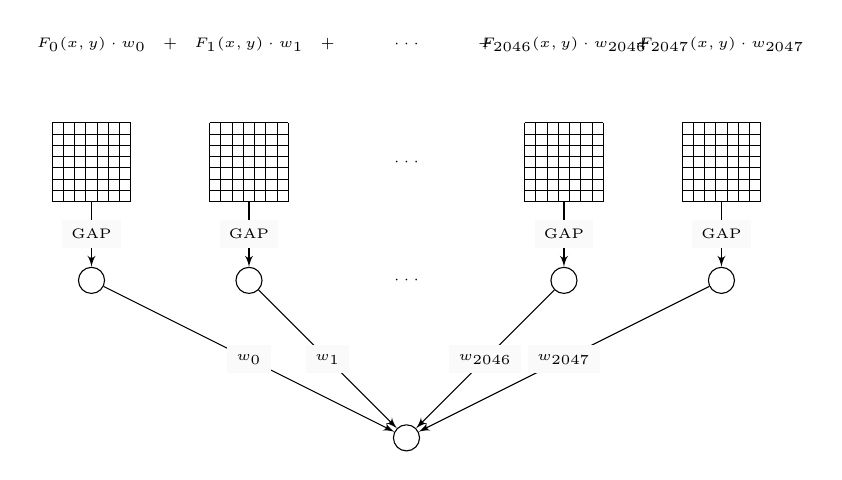
\begin{tikzpicture}[auto, node distance = 3cm, > = latex', font = \tiny]
    \tikzset{
      neuron/.style = {draw, circle},
      weight/.style = {fill = black!2, anchor = center},
    }

    \node [neuron] (output) at (0, -1) {};
    \node [neuron] (gap0) at (-4, 1) {};
    \node [neuron] (gap1) at (-2, 1) {};
    \node (gap2) at (0, 1) {$\cdots$};
    \node [neuron] (gap3) at (2, 1) {};
    \node [neuron] (gap4) at (4, 1) {};

    \draw [->] (gap0) -- node[weight]{$w_{0}$} (output);
    \draw [->] (gap1) -- node[weight]{$w_{1}$} (output);
    \draw [->] (gap3) -- node[weight]{$w_{2046}$} (output);
    \draw [->] (gap4) -- node[weight]{$w_{2047}$} (output);

    \draw[step = 0.142857143, shift = {(-4.5, 2)}] (0, 0) grid (1, 1);
    \draw[step = 0.142857143, shift = {(-2.5, 2)}] (0, 0) grid (1, 1);
    \node at (0, 2.5) {$\cdots$};
    \draw[step = 0.142857143, shift = {(1.5, 2)}] (0, 0) grid (1, 1);
    \draw[step = 0.142857143, shift = {(3.5, 2)}] (0, 0) grid (1, 1);

    \draw [->] (-4, 2) -- node[weight]{GAP} (gap0);
    \draw [->] (-2, 2) -- node[weight]{GAP} (gap1);
    \draw [->] (2, 2) -- node[weight]{GAP} (gap3);
    \draw [->] (4, 2) -- node[weight]{GAP} (gap4);

    \node (term0) at (-4, 4) {$F_0(x, y) \cdot w_0$};
    \node (term1) at (-2, 4) {$F_1(x, y) \cdot w_1$};
    \node (term2) at (0, 4) {$\cdots$};
    \node (term3) at (2, 4) {$F_{2046}(x, y) \cdot w_{2046}$};
    \node (term4) at (4, 4) {$F_{2047}(x, y) \cdot w_{2047}$};

    \node (add01) at (-3, 4) {$+$};
    \node (add12) at (-1, 4) {$+$};
    \node (add23) at (1, 4) {$+$};
    \node (add34) at (3, 4) {$+$};
  \end{tikzpicture}
  \end{center}
  \caption{
    An illustration of the CAM equation for binary classification.
  }
  \label{fig:CAMIllustration}
  \end{figure}
\end{frame}

\begin{frame}{Example CAM}
  \begin{figure}
  \begin{center}
    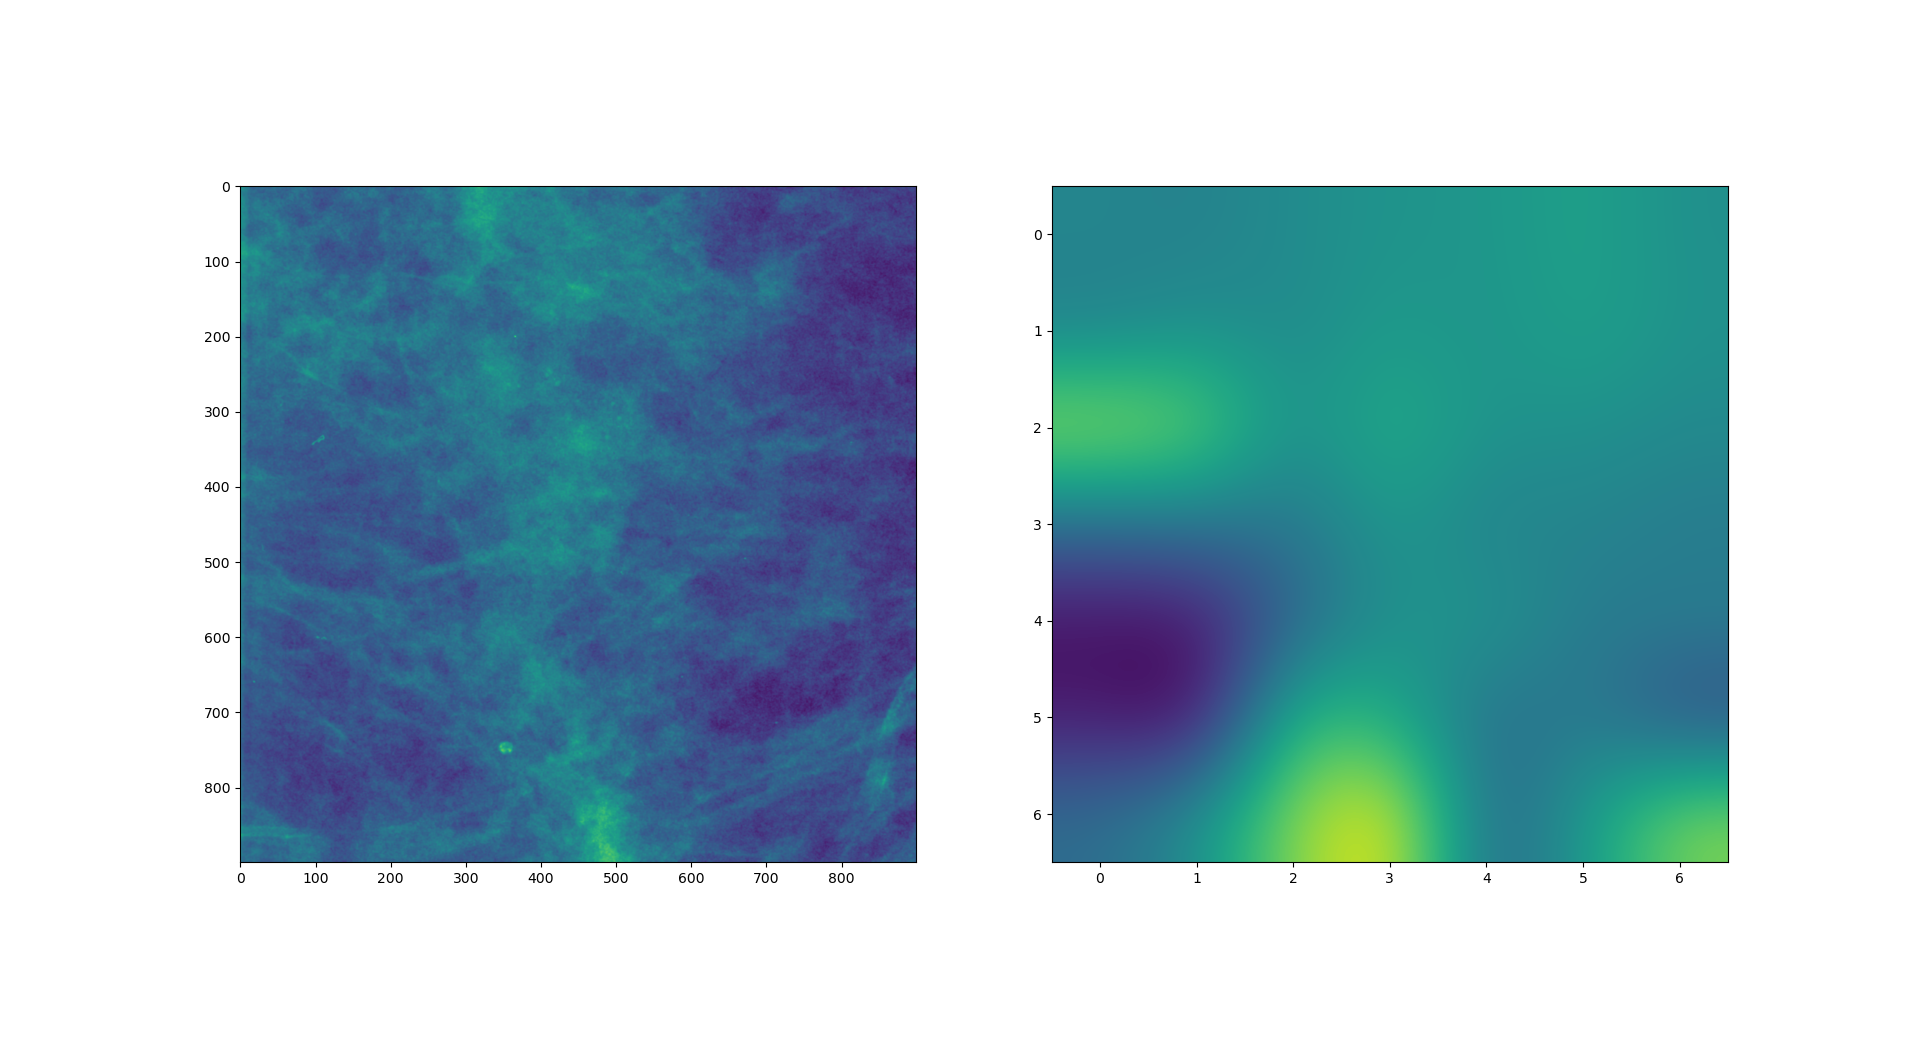
\includegraphics[width=\textwidth]{../docs/classActivationMap}
  \end{center}
  \caption{An example class activation map for a mammogram with a mass. Bright
    areas denote higher significance.}
  \label{fig:ClassActivationMap}
  \end{figure}
\end{frame}

\section{Conclusion}

\begin{frame}{Conclusion}
  \begin{itemize}
    \item Our implantation of the paper achieved a binary accuracy of
      \alert{77\%} on the testing dataset.
    \item This is a much lower accuracy compared to the results of the paper.
    \item This is likely due to the corners we cut when it comes to fine tuning
      the model and the use of a smaller dataset.
  \end{itemize}
\end{frame}

\section{References}

\begin{frame}[allowframebreaks]{References}
  \printbibliography[heading=none]
\end{frame}

\end{document}
